\section{Application in a Design Context}
When having used the framework for analysis, it is clear that use in a design context would not be constructive, since the complexity necessitates a high degree of absorption and, most importantly, loads of time. Therefore, for the creation of a practical method, I decided to delegate the effort into two parts taking place during well-known processes in game development: Playtesting and ideation. To test the effectiveness of the proposed method I gathered a group of experienced game developers who, importantly, have not undertaken the same education specialisation as me, which assisted the developing of a universal method, and avoiding a method specific for game developers out of a narrow school of thought. Another beneficial of the test group was that they had previously worked on games together which limited the amount of noise arising from not knowing each others' approaches to game development, and assuring a solid baseline for comparison to previous development situations. The testing was separated into three phases corresponding to the two processes of playtesting and ideation. First phase consisted of a playtesting situation with a prototype video game made by me specifically for the test, me acting as the interviewer and each group member sequentially acting as the playtester. Second phase consisted of the group being presented to a drawn model on a whiteboard representing the simplified framework and the data I had gathered from the playtest. Third and last phase consisted of a semi-structured focus group interview \cite{cresswell} where the participants had a chance to discuss their impressions. The method for gathering qualitative data was chosen to be a focus group because the relevant feedback was identified as being impressions from a development group since this was the pursued target of the method.

The main goal of the prototype video game was for it to be used as a tool for evaluating the proposed method, so the most important aspect was identified as the prototype aspiring to be as original as possible. The intend of this were to disconnect previous experiences the test participants might have had if the prototype had been similar to a game they had played previously, thereby optimistically limiting unknown variables in the evaluation. Realising creating something original is a perilous task, emphasis was simply put on implementing as few as possible conventional game mechanics such as using the W, A, S and D key for movement. Consequently, movement in the prototype is controlled by a mouse-wheel with the playable figure also resembling this wheel (see figure \ref{prototype}). The prototype consists of three minor challenges to ground the player in the control scheme and one integral kinaesthetic challenge as the focus of the test. This kinaesthetic challenge can be seen in figure \ref{prototype}. It consists of two doorways, one from which the player enters and the other through which the player needs to exit. Between the two doorways is a lowered area creating a gap between the two which makes travelling from one doorway directly to the other impossible since the playable figure cannot inherently move vertically. Leaning on the pathway leading into the room is a large barrel oriented horizontally which is suspended off the lower ground by a round beam going through the barrel's centre. The beam is held up by its extremities lying in two grooves in the walls perpendicular to the doorways. Lastly, the room is sloping toward the entrance making the entrance level slightly lower than the exit. The intended strategy to get to the other side is then to position the playable figure, a wheel, on top of the barrel and then use the weight of the wheel to rotate the barrel, which rotates the beam which progresses everything forward towards the exit where the player can climb off the barrel and exit.

\begin{figure}[h]
  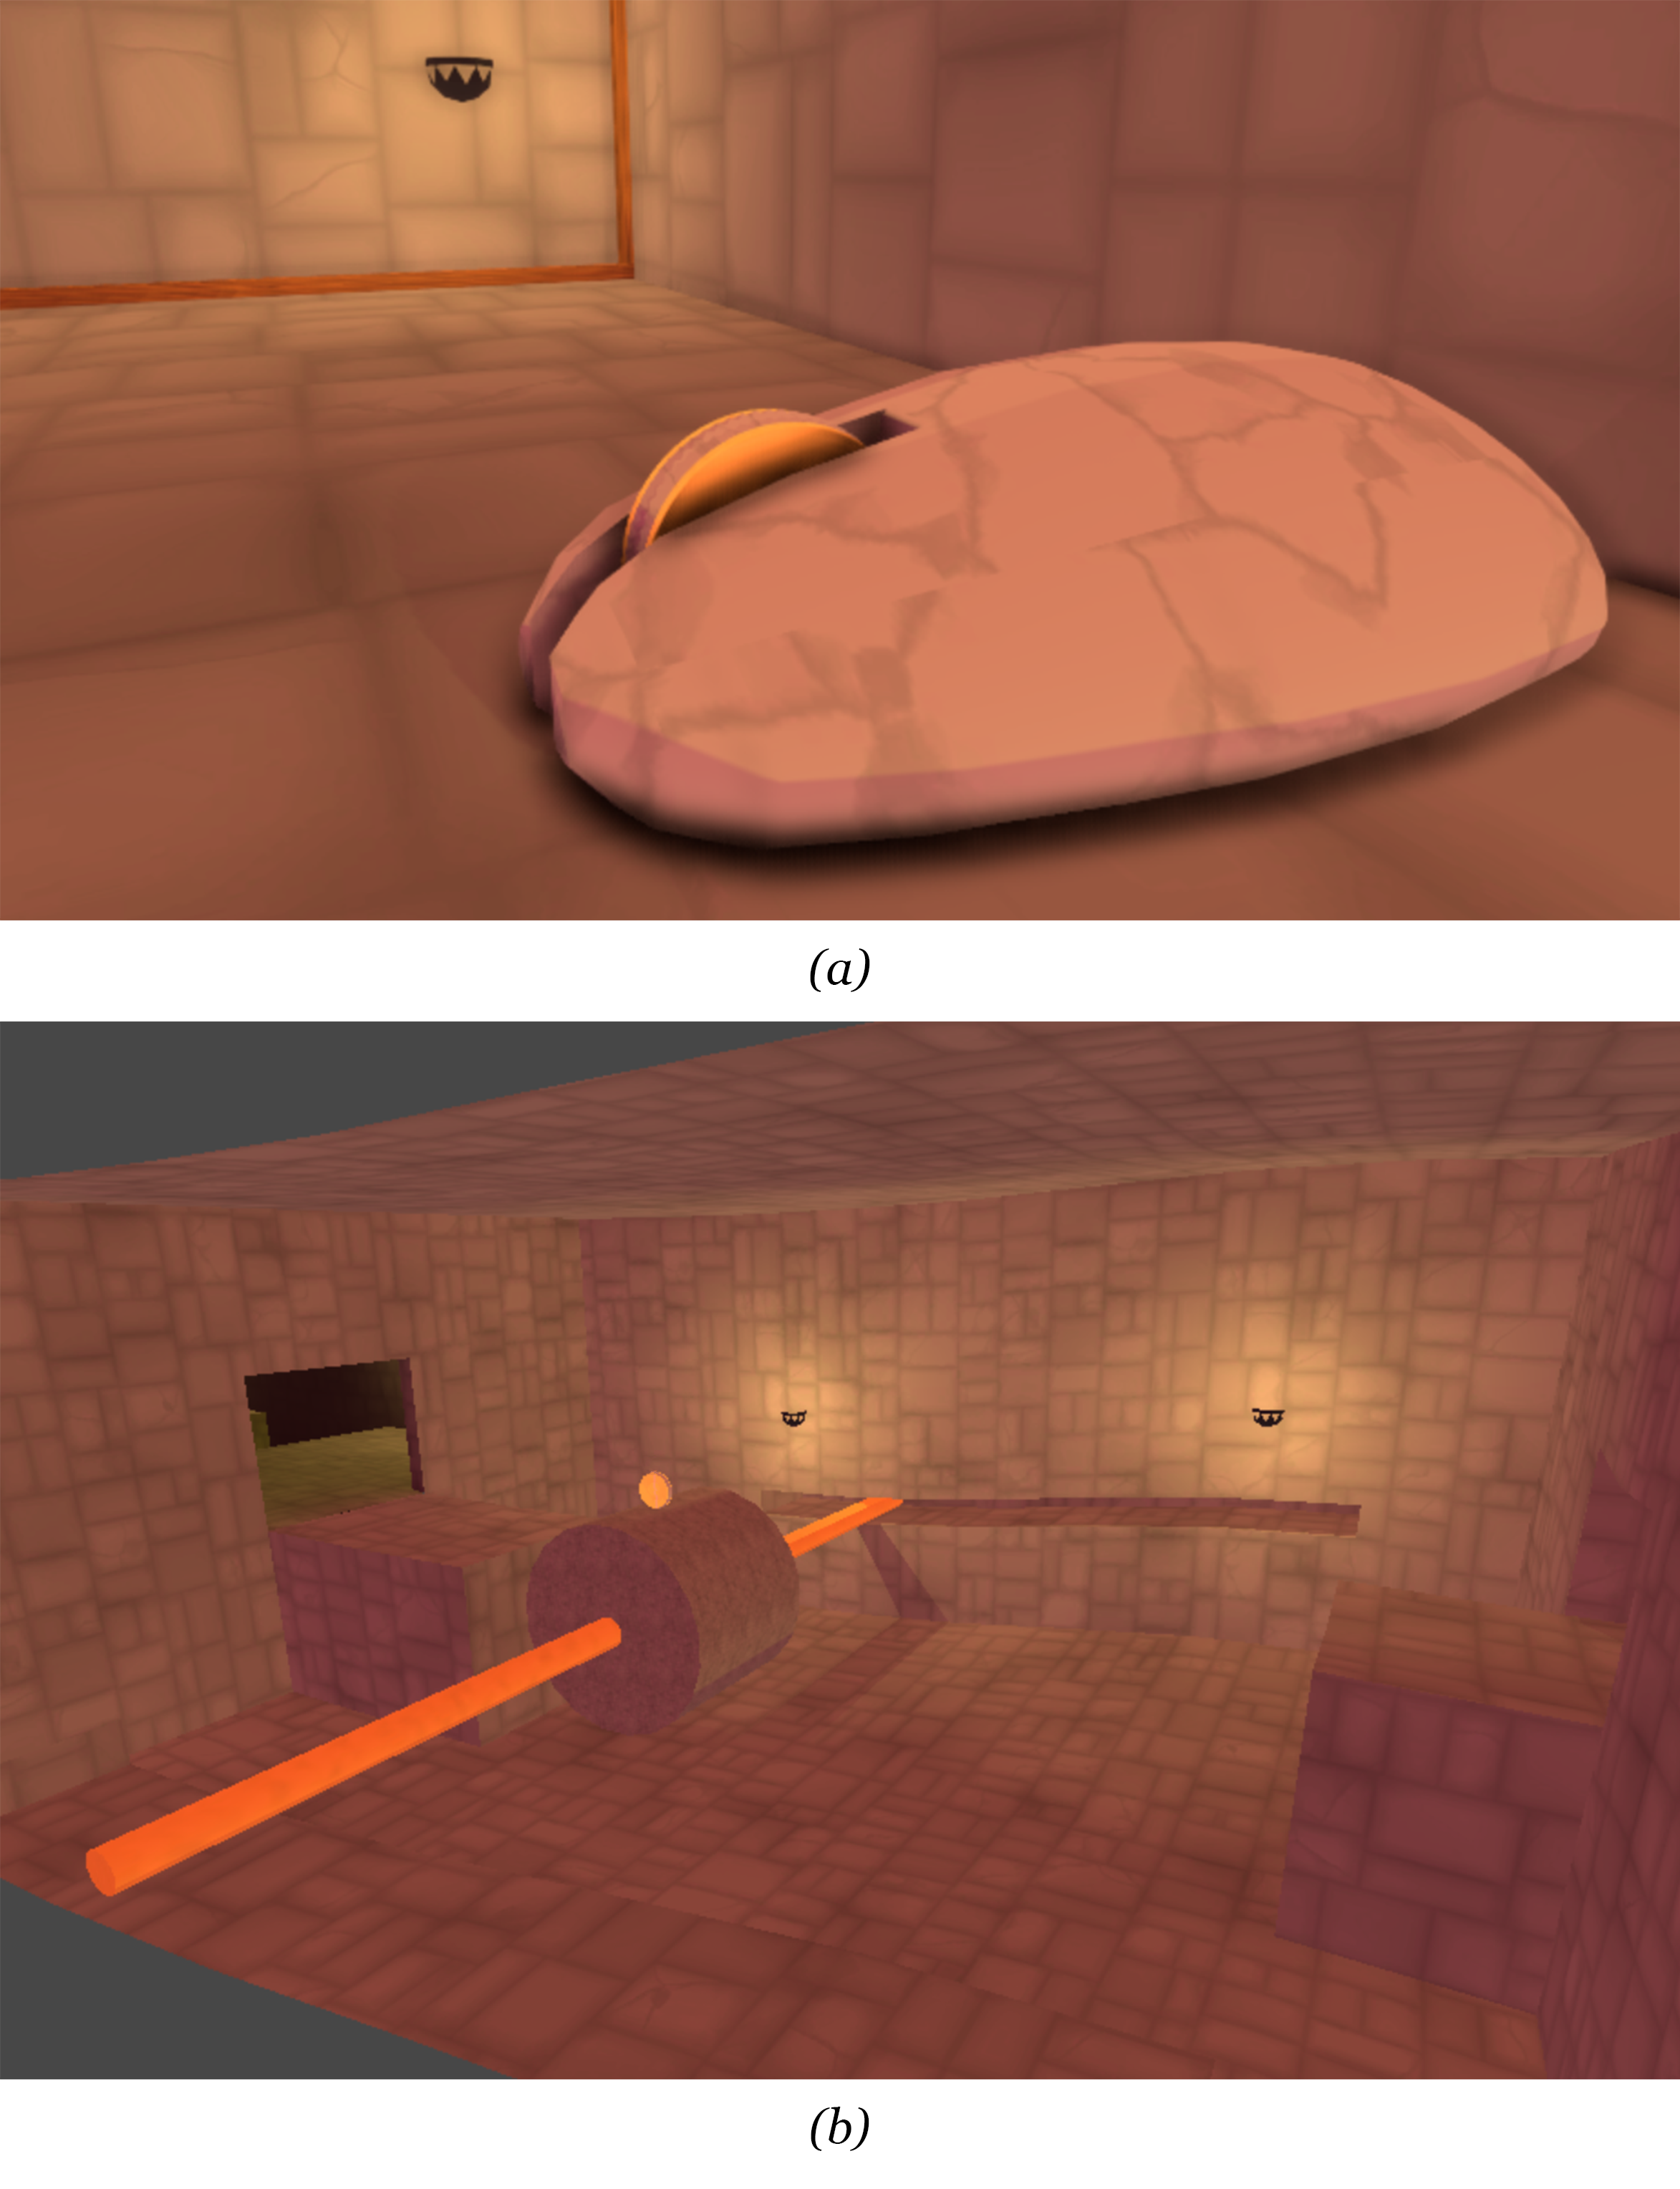
\includegraphics[width=\textwidth]{PrototypeBoth}
  \caption{(a) In-game photo of the prototype as it is presented to a new player (b) The kinaesthetic challenge in focus}
  \label{prototype}
\end{figure}

Summing up, the described challenge acted as the focus point of the application phases of playtesting and ideation while the method as a whole was the focus of the last evaluating phase with the focus group interview. The next two sections will address the substance of the proposed method and the relevant findings during the two first phases of application and the impressions of the participants from the last evaluating phase.

\subsection{Playtesting}
The workload of identifying relevant information regarding the six aspects of time, location, direction, modality, dynamics and expression from the framework has been delegated to a playtesting phase in the simplified method. The way this is done is that the interviewer conducting the playtest adhere to a number of questions during the playtest. The questions are divided in two parts: Before the identified challenge is attempted and right after. These two phases reflects the phases of pre-action and post-action in the framework and is thereby related to perceivable feedforward and feedback. The questions have been formulated to echo the six aspects in a feedforward setting and a feedback setting and is preluded by a contextual question limiting the scope of the following questions totalling the questions to 14. Each question is, additionally, asked with relevance to both the physical world and the game world, so each question can be said to be two-fold, thereby covering the two dimensions of the framework.

\begin{enumerate}
  \item \textbf{Feedforward}
  \begin{enumerate}
    \item What action would you invoke to overcome the challenge?
    \item When would you apply this action and when would you stop?
    \item Where would you apply this action?
    \item In what direction would you apply this action?
    \item Is there something visually, audibly or tangibly that instructs you how to apply this mechanic?
    \item How much force, speed or acceleration do you think you need to apply?
    \item Do you think you need to apply a certain kind of attitude when applying the action?
  \end{enumerate}
  \item \textbf{Feedback}
  \begin{enumerate}
    \item Now that you have invoked the action, do you feel it was effective in overcoming the challenge?
    \item Did you feel that the action and the effect happened synchronously?
    \item Did you feel that the action and the effect happened at the same location?
    \item Did you feel that the direction of the action was parallel to the direction of the effect?
    \item Did you feel that there was any visual, tactile or audible feature that arose as a consequence of you action?
    \item Did you feel that the amount of force/speed/acceleration from your action was apparent in the effect?
    \item Did you feel that the attitude you applied in your action was apparent in the effect?
  \end{enumerate}
\end{enumerate}

As the questions were formulated they were evaluated by using them in the context they were designed for, a playtest. The focus of the playtest, was as discussed earlier, the challenge in the constructed prototype. The way the playtesting was conducted was that I sat down with each participant separately and let them play through the first three minor challenges without instructing them in anything other than letting them know that at a point I would stop them and ask them some questions. As the playtesting participant reached the challenge in focus I asked them to halt the movement of the playable figure and allowed them to look around in the game world without progressing the challenge. With the game still running I went through the first seven questions in order, waiting for the participant to answer each accordingly. Each question was additionally followed up by a request for elaboration, mostly by asking why they answered what they did. As the participants answered I wrote down their answers in the form of notes with the intend of the notes being the collected data to be used in the ideation phase. As the final question was discussed I gave back the reins with the encouragement of applying the action they answered the first question with. If the action was successful in overcoming the challenge I carried on with the last seven questions, if not I asked the first seven questions once more, this time the participant having gained new knowledge.

What was clear from the perspective of the interviewer was that the universal nature of the questions lead to some of the questions seeming trivial. As an example, when inquiring with the questions regarding time (1b and 2b), as an interviewer, I was awaiting an affirmative answer, not expecting any other reply, and as a consequence a feeling of the question as being unconstructive arose. This same consideration was also voiced during the focus group interview. Here, the participants suggested that the playtesting interview be conducted in a semi-structured way with the questions acting as a starting point but as the interview goes on the interviewer follows the flow of conversation. This suggestion, in addition with a suggestion of digging even deeper in elaboration on some questions like dynamics and modality (1e, 1f, 2e and 2f), I welcome. What is apparent from the test is that the questions should be considered a checklist to be answered through relevant discussion between the interviewer and the playtester in no particular order other than the first question in each section being first. With that said, this alteration requires diligence of the interviewer since the task of categorising the data becomes more complex, but most importantly keeping on-topic becomes of high importance. It is of course possible to disregard these two tasks, but let me provide one argument for each task for why they should not: (1) The task of categorisation should not be disregarded because the categorisation inherently provides information on where a weakness or a strength in the design lies and if disregarded can lead to designers focusing on coupling on an aspect that is inappropriate for what the playtester actually experienced. Vice versa, the task of categorisation could be given to the designers, leaving them to code the data \cite{cresswell}. What is inappropriate with this approach is that tacit knowledge from the actual playtesting situation is lost \cite{cresswell}. Conclusively, I suggest that the categorisation task should be prioritised and should be conducted by the interviewer as close in time to the playtesting as possible. (2) The task of keeping on-topic should not be disregarded because the scope of the method is relatively narrow. What can happen if the subject matter is deprioritised is that the playtesting session can evolve into a general playtesting session with discussions concerning graphical glitches, similarities to other games, aesthetic qualities, etc. which can end up being irrelevant for the purpose of the playtest, which is to gather data on the intuitiveness of a kinaesthetic challenge.

One other interesting finding was the difficulty of the participants to express and identify what they felt and why they felt the way they did. This lead to interesting replies such as when asked how much force, speed or acceleration they thought they would need to apply in the context of scrolling the mouse wheel fast enough to use the barrel as a ramp for the playable figure the participant answered that he thought he would need as much force as one would apply to get to the bottom of a webpage. This can be explained by the fact that the method, as well as the framework, is highly concerned with knowledge residing in the lebenswelt \cite{dourish}: The intersubjective unconscious knowledge and understandings gained from experience. This knowledge is tacit knowledge in the way that it is hard to explain to another person. What makes this example so important is that intersubjectivity is used to answer the question in a way that many people would understand because most people have experienced the situation of wanting to scroll to the bottom of a page: It is forceful and fast. From this finding, I suggest that any utilisation of the proposed method include an explanation from the interviewer in the playtesting processes of the possibility of using past experiences as examples to identify what is felt and how it is felt.

\subsection{Sketching}
Why did I collapse the information? holistic

``The differentiation between the three different types of feedforward was mainly made for analysis purposes (citing personal communication with Wensveen)'' \cite[p. 5]{vermeulen}.

``Their value lies not in the artifact of the sketch itself, but in its ability to provide a catalyst to the desired and appropriate behaviors, conversations, and interactions'' \cite[p. 113]{buxton}.

During the lecture I mirrored \cite{frogger} in saying that inherent information is better than augmented because of psychomotor vs cognitive.


Coupling, strengthening, analysing and decoupling.
Feedback: Amplify or reduce
Feedforward: Invite or inhibit












Use: See if there's any other game mechanics that need decoupling or the correct game mechanic needs strengthening OR to embrace the coupling and make it a possibility.

 Multiple strategies. The Deku Baba can be killed in a number of ways. This means rich interaction.

 Inherent is preferred because it requires less attention, thereby helping in internalising controls \cite{calleja}.
